\documentclass[4paper]{article}
\usepackage[spanish]{babel}
%\usepackage[ansinew]{inputenc}
\usepackage[utf8x]{inputenc}
%\usepackage[utf-8]{inputenc}
%\usepackage[T1]{fontenc}
\usepackage{graphicx}
\usepackage{multicol}
\usepackage{float}
\usepackage{hyperref} 
%\usepackage{longtable}
%\usepackage{array}
%\usepackage{multirow}
%\usepackage[latin1]{inputenc}
%\inputencoding{latin}
\newcommand{\J}{Java}
\newcommand{\p}{procesos}
\newcommand{\s}{procesos}

%\newcommand{\j}{JavaScript }
%%%%%%%%%%%%%%%%%%%%%%%%%%%%%%%%%%%%%
%Para escribir codigo en latex
\usepackage{listings}
\usepackage{color}

\definecolor{lightgray}{rgb}{.9,.9,.9}
\definecolor{darkgray}{rgb}{.4,.4,.4}
\definecolor{purple}{rgb}{0.65, 0.12, 0.82}

\lstdefinelanguage{JavaScript}{
  keywords={typeof, new, true, false, catch, function, return, null, catch, switch, var, if, in, while, do, else, case, break},
  keywordstyle=\color{blue}\bfseries,
  ndkeywords={class, export, boolean, throw, implements, import, this},
  ndkeywordstyle=\color{darkgray}\bfseries,
  identifierstyle=\color{black},
  sensitive=false,
  comment=[l]{//},
  morecomment=[s]{/*}{*/},
  commentstyle=\color{purple}\ttfamily,
  stringstyle=\color{red}\ttfamily,
  morestring=[b]',
  morestring=[b]"
}

\lstset{
   language=JavaScript,
   backgroundcolor=\color{lightgray},
   extendedchars=true,
   basicstyle=\footnotesize\ttfamily,
   showstringspaces=false,
   showspaces=false,
  % numbers=left,
   numberstyle=\footnotesize,
   numbersep=9pt,
   tabsize=2,
   breaklines=true,
   showtabs=false,
   captionpos=b
}
%%%%%%%%%%%%%%%%%%%%%%%%%%%%%%%%%%%%%%%%
\renewcommand{\tablename}{Tabla}
\renewcommand{\S}{ \p}
\author{Manuel Molino Milla}
\title{\textbf{MongoDB}}
\date{\today}

\begin{document}
\maketitle 
\tableofcontents
\newpage

\section{Introducción}

\subsection{NoSQL}
\begin{itemize}
\item Es una amplia clase de sistemas de gestión de bases de datos que difieren del modelo clásico de SGBDR (Sistema de Gestión de Bases de Datos Relacionales).
\item No usan SQL como lenguaje principal de consultas.
\item Los datos almacenados no requieren estructuras fijas como tablas.
\item Los sistemas de bases de datos NoSQL crecieron con las principales redes sociales.
\item Con el crecimiento de la web en tiempo real existía una necesidad de proporcionar información procesada a partir de grandes volúmenes de datos que tenían unas estructuras horizontales más o menos similares. 
\item Estas compañías se dieron cuenta de que el rendimiento y sus propiedades de tiempo real eran más importantes que la coherencia, en la que las bases de datos relacionales tradicionales dedicaban una gran cantidad de tiempo de proceso.
\end{itemize}

\subsection{SQL/NoSQL}
En las bases de datos relacionales, los datos se almacenan en diferentes tablas, generelmente conectadas usando claves primarias y foráneas.\\
Usando lenguaje SQL insertas, recuperas, borras o actulizas datos.\\
En NoSQL se denominan base de datos orientadas a documentos, almacenados en formatos estándar tales como JSON o XML.\\
Ejemplo de BD SQL:
\begin{figure}[H]
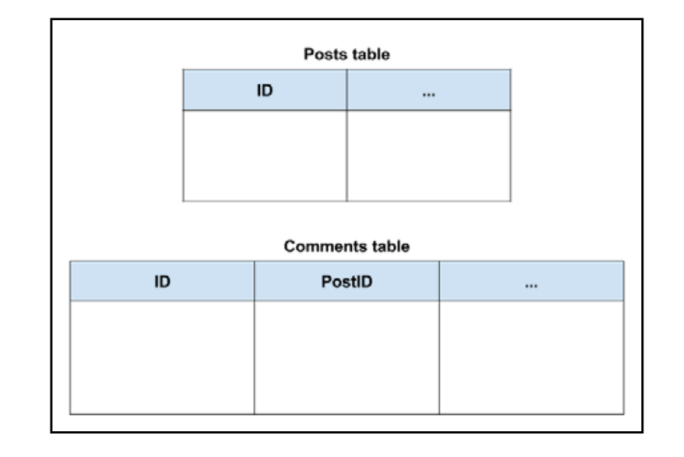
\includegraphics[scale=0.5]{sql.png}
\end{figure}
Ejemplo de BD NoSQL:
\begin{lstlisting}
{
   "title": "First Blog Post",
   "comments": [......, ......]
}
\end{lstlisting}
Otro problema es la escalabilidad, \emph{¿qué ocurre si añadimos una nueva propiedad?}

\subsection{BD NoSQL}
\begin{itemize}
\item MongoDB.
\item Cassandra.
\item Redis.
\item CouchDB.
\end{itemize}

\section{MongoDB}
\subsection{Introduccion}
\begin{itemize}
\item Es un sistema de base de datos NoSQL orientado a documentos, desarrollado bajo el concepto de código abierto.
\item MongoDB guarda estructuras de datos en documentos similares a JSON 
\item MongoDB utiliza una especificación llamada BSON (Binary JSON)
\item El desarrollo de MongoDB empezó en octubre de 2007 por la compañía de software \textit{10gen}.
\item Los drivers para los lenguajes de programación están bajo la licencia de Apache. 
\item MongoDB está escrito en C++, aunque las consultas se hacen pasando objetos JSON como parámetro.
\end{itemize}



\subsection{¿Dónde se puede utilizar MongoDB?}
\begin{itemize}
\item Cualquier aplicación que necesite almacenar datos semi estructurados puede usar MongoDB.
\item Es el caso de las típicas aplicaciones CRUD de muchos de los desarrollos web actuales.
\item MongoDB es especialmente útil en entornos que requieran escalabilidad. 
\end{itemize}

\subsection{¿Dónde no se debe usar MongoDB?}
\begin{itemize}
\item En esta base de datos no existen las transacciones. Solo garantiza operaciones atómicas a nivel de documento.Si las transacciones son algo indispensable en nuestro desarrollo, deberemos pensar en otro sistema.
\item Tampoco existen los JOINS. Para consultar datos relacionados en dos o más colecciones, tenemos que hacer más de una consulta. En general, si nuestros datos pueden ser estructurados en tablas, y necesitamos las relaciones, es mejor que optemos por un RDBMS clásico.
\end{itemize}


\section{Instalación}

\href{https://docs.mongodb.com/manual/administration/install-community/}{Instalación mongodb}

\section{Manejo MongoDB}
\subsection{Database}
\begin{LARGE}
Un registro en MongoDB es un documento.\\

\end{LARGE}El cual es un estructura de datos compuesto por un campo y un valor, estos documentos son similares a los objetos JSON. Los valores de los campos pueden incluir otros documentos, arrays o arrays de documentos.

\begin{figure}[H]
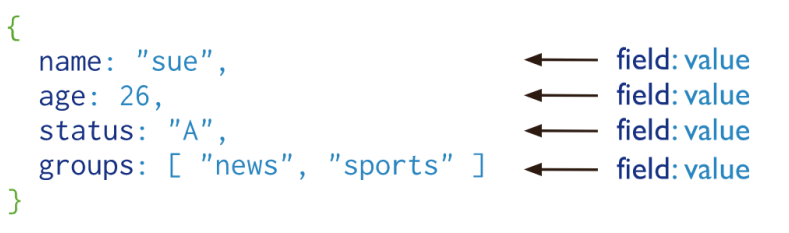
\includegraphics[scale=0.5]{documentos.png}
\end{figure}

Los documentos son almacenados en colecciones:
\begin{figure}[H]
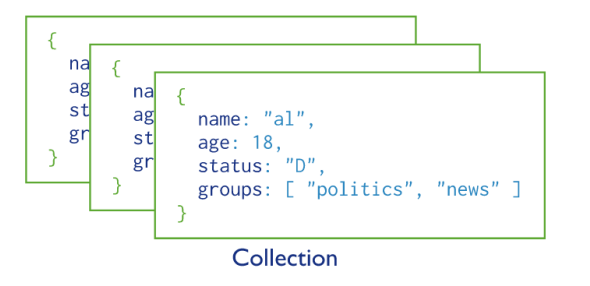
\includegraphics[scale=0.5]{colecciones.png}
\end{figure}
Y las colecciones en base de datos\\
\begin{center}
\begin{Large}
\textit{En MongoDB, las bases de datos almacenan colecciones de documentos.}
\end{Large}
\end{center}

Cada servidor mongo puede almacenar muchas bases de datos, por defecto se conecta a la base de datos denominada \emph{test}\\
Para crear una nueva base de datos, en la shell de mongo hacemos:
\begin{quote}
\textit{use bd
}\end{quote}
Podemos entrar directamente con:
\begin{quote}
\textit{mongo bd}
\end{quote}
Podemos conocer las bases de datos del servidor con:
\begin{quote}
\textit{show dbs}
\end{quote}
Existen \href{https://docs.mongodb.com/manual/reference/limits/#restrictions-on-db-names}{restricciones al nombre de las bases de datos}

\subsubsection{Documentos MongoDB}
Los datos se almacenan en documentos \emph{BSON} que es una representación binaria  de documentos \emph{JSON}
\begin{figure}[H]
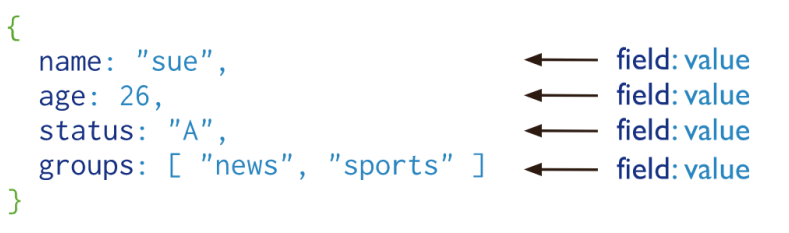
\includegraphics[scale=0.5]{documentos.png}
\end{figure}
\begin{lstlisting}
var mydoc = {
               _id: ObjectId("5099803df3f4948bd2f98391"),
               name: { first: "Alan", last: "Turing" },
               birth: new Date('Jun 23, 1912'),
               death: new Date('Jun 07, 1954'),
               contribs: [ "Turing machine", "Turing test", "Turingery" ],
               views : NumberLong(1250000)
            }
\end{lstlisting}
En cuanto a \href{https://docs.mongodb.com/manual/reference/bson-types/}{tipos de datos}

Restricciones en el nombre de los campos:
\begin{itemize}
\item El campo \_id está reservado para us de \emph{primary key}; 
\item El campo no puede empezar por \$.
\item Tampoco puede contener el punto (.)
\item Ni ningún caracter nulo.
\end{itemize}


\subsection{MongoDB CRUD}
Las operaciones CRUD son \emph{create, read, update y delete}\\
\subsubsection{Create}
Tenemos el método:
\begin{itemize}
\item db.collection.insert() 
\end{itemize}
%\begin{figure}[H]
%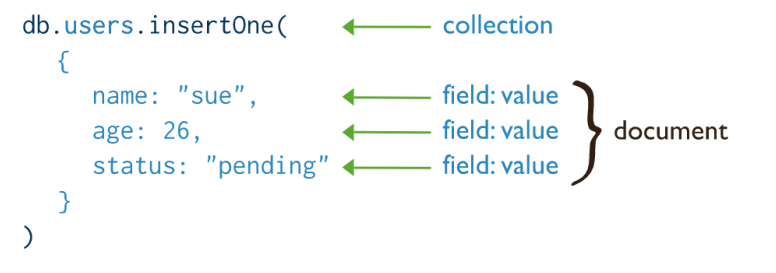
\includegraphics[scale=0.5]{insert1.png}
%\end{figure}
\begin{large}
\textbf{Insertando un registro}
\end{large}
\begin{lstlisting}
db.inventory.insert(
   { item: "canvas", qty: 100, tags: ["cotton"], size: { h: 28, w: 35.5, uom: "cm" } }
)
\end{lstlisting}


\subsubsection{Read}
\begin{quote}
db.collection.find()
\end{quote}
\begin{figure}[H]
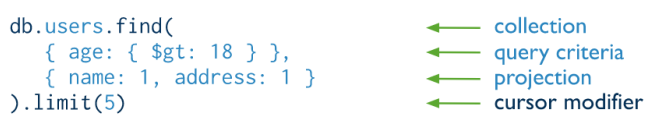
\includegraphics[scale=0.5]{query.png}
\end{figure}
\begin{lstlisting}
db.inventory.find( {} )
SELECT * FROM inventory

db.inventory.find( { status: "D" } )
SELECT * FROM inventory WHERE status = "D"

db.inventory.find( { status: { $in: [ "A", "D" ] } } )
SELECT * FROM inventory WHERE status in ("A", "D")

db.inventory.find( { status: "A", qty: { $lt: 30 } } )
SELECT * FROM inventory WHERE status = "A" AND qty < 30

db.inventory.find( { $or: [ { status: "A" }, { qty: { $lt: 30 } } ] } )
SELECT * FROM inventory WHERE status = "A" OR qty < 30

db.inventory.find( {
     status: "A",
     $or: [ { qty: { $lt: 30 } }, { item: /^p/ } ]
} )
SELECT * FROM inventory WHERE status = "A" AND ( qty < 30 OR item LIKE "p%")

db.inventory.find( { status: "A" }, { item: 1, status: 1 } )
SELECT _id, item, status from inventory WHERE status = "A"

db.inventory.find( { status: "A" }, { item: 1, status: 1, _id: 0 } )
SELECT item, status from inventory WHERE status = "A"
\end{lstlisting}


\subsubsection{Update}
\begin{itemize}
\item db.inventory.update()
\end{itemize}
\begin{lstlisting}
db.users.update(
   { name: "xyz" },
   { name: "mee", age: 25, type: 1, status: "A", favorites: { "artist": "Matisse", food: "mango" } }
)
\end{lstlisting}
La sintáxis mas compleja es:
\begin{lstlisting}
db.collection.update(
   <query>,
   <update>,
   {
     upsert: <boolean>,
     multi: <boolean>,
     writeConcern: <document>
   }
)
\end{lstlisting}
Donde:
\begin{description}
\item[query] Es el criterio de selección.
\item[update] El modificador a aplicar.
\item[upsert] En caso de la opción \emph{true}, si no hay ningún documento que cumpla las codificiones de búsqueda, se crea un nuevo documento.
\item[multi] En el caso de la opción \emph{true} se modifica NO solo el primero que cuple la condición de búsqueda, se modifican TODOS.
\end{description}

\newpage
Ejemplo:
\begin{lstlisting}
db.people.update(
   { name: "Andy" },
   {
      name: "Andy",
      rating: 1,
      score: 1
   },
   { upsert: true }
)

db.collection.update( { "_id.name": "Robert Frost", "_id.uid": 0 },
   { "categories": ["poet", "playwright"] },
   { upsert: true } )
   

db.books.update(
   { _id: 1 },
   {
     $inc: { stock: 5 },
     $set: {
       item: "ABC123",
       "info.publisher": "2222",
       tags: [ "software" ],
       "ratings.1": { by: "xyz", rating: 3 }
     }
   }
)

db.mycol.update({'title':'MongoDB Overview'},
   {$set:{'title':'New MongoDB Tutorial'}},{multi:true})   
\end{lstlisting}
El modificador \emph{\$inc} es de incremento y \emph{\$set} para la nueva condición 
\subsubsection{Delete}
Borrado de una colección completa:
\begin{itemize}
\item db.collection.remove().
\end{itemize}
%\begin{figure}[H]
%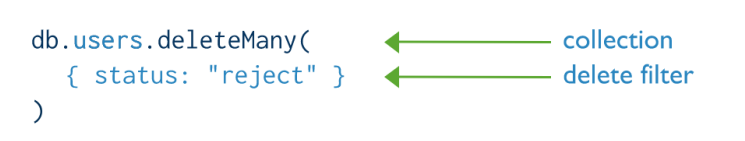
\includegraphics[scale=0.5]{delete.png}
%\end{figure}
Borrado de un documento:
\begin{verbatim}
db.users.remove( { status: "D" }, 1)
\end{verbatim}

\newpage
\subsubsection{Ejemplos de relacion entre SQL y NoSQL}
Creacion de tablas:
\begin{lstlisting}
CREATE TABLE people (
    id MEDIUMINT NOT NULL
        AUTO_INCREMENT,
    user_id Varchar(30),
    age Number,
    status char(1),
    PRIMARY KEY (id)
)

db.people.insert( {
    user_id: "abc123",
    age: 55,
    status: "A"
 } )
 
db.createCollection("people") (se crea la coleccion vacia)
\end{lstlisting}
\newpage
Añadimos una nueva columna a la tabla:
\begin{lstlisting}
ALTER TABLE people
ADD join_date DATETIME

db.people.update( 
  { },
  { $set: {join_date : new Date() }},
  {multi: true}
)
\end{lstlisting}
\vspace{0.5cm}
Borrado de una columna:
\begin{lstlisting}
ALTER TABLE people
DROP COLUMN join_date

db.people.update( 
  { },
  { $unset: {join_date : '' }},
  {multi: true}
)
\end{lstlisting}
\vspace{0.5cm}
Creación de índice:
\begin{lstlisting}
CREATE INDEX idx_user_id_asc
ON people(user_id)

db.people.createIndex( { user_id: 1 } )

CREATE INDEX
       idx_user_id_asc_age_desc
ON people(user_id, age DESC)

db.people.createIndex( { user_id: 1, age: -1 } )
\end{lstlisting}
\vspace{0.5cm}
Borrado de una tabla
\begin{lstlisting}
DROP TABLE people

db.people.drop()
\end{lstlisting}

\vspace{1cm}
{\LARGE \href{https://www.tutorialspoint.com/mongodb/}{Tutorial de tutorialpoins}}

\newpage
\subsubsection{Ejercicio}
\begin{itemize}
\item Busca informacion de como importar una colección a una base de datos de \emph{mongodb} a partir de un fichero conteniendo un array \emph{json} (Usa el fichero \emph{personas.json})
\item Incorpora un documento con tus datos personales.
\item Busca todos los documentos relacionados con objetos que tenga el mismo valor que tu edad.
\item Busca todos los documentos que correspondan a persona mayores de edad.
\item Ahora todos los documentos que correspondan a persona menores de edad y sexo femenino.
\item Igual que antes y además que su nombre debe comenzar por A
\item Igual que antes y además que su nombre debe comenzar por A o por F.
\item Cambia de sexo al docuento que corresponde a tus datos personales.
\item Cambia a sexo \emph{Male} a todos los documentos que corresponde a menores de edad.
\item Añade una nueva columna, denominada fecha y cuyo valor sea la fecha actual.
\item Busca información de como exportar los datos de la colección anterior teniendo en cuenta:
\begin{itemize}
\item Queremos guardar 100 documentos.
\item Para aquellos que sean mayores de edad.
\item Empezando por el registro 200
\end{itemize} 
\end{itemize}




\end{document}
